\chapter{Evaluation}
\label{cha:ExperimentalDesign}
This chapter describes the experimental design for two evaluation tasks: (1) applying the evaluation framework described in \autoref{cha:framework-description} to the Makahiki system described in \autoref{cha:system-description}, (2) applying the same evaluation framework to a second IT infrastructure for serious games for sustainability.

To applying the evaluation framework described in \autoref{cha:framework-description}, we propose to investigate the following research questsions:

\begin {itemize}
    \item \emph{To what extent does the system effectively enage players?}
    \item \emph{To what extent does the system effectively increase player's literacy in sustainability}
    \item \emph{To what extent does the system effectively produce positive player behavior change in sustainability?}
    \item \emph{How efficient is it to design a game using the system?}
    \item \emph{How efficient is it to manage the game using the system?}
    \item \emph{How efficient is it to install and maintain the system?}
    \item \emph{How efficient is it to understand, extend and debug the system?}
    \item \emph{How efficient is it to do research with the system?}
\end {itemize}

\section{Makahiki Evaluation}
I propose to evaluate the Makahiki system in two ways: (1) case studies of Makahiki instances in real-world, namely the three Kukui Cup serious games deployed in University of Hawaii at Manoa, Hawaii Pacific University, and East West Center of Hawaii. (2) in-lab experiement of evaluting Makahiki system by the students taking the serious game development course in the Universiy of Hawaii at Manoa.

\subsection{Real-world Makahiki Case Studies}

Using the Makahiki as the IT infrastructure, the first and second Kukui Cup Energy challenge of University of Hawaii was held in 2011 and 2012 for over 1,000 first year students living in the residence halls. Hawaii Pacific University (HPU) held a Kukui Cup Energy challenge in Fall 2012 for about 200 students. An international organization called the East-West Center (EWC) held a Kukui Cup Energy and Water challenge for the international residents living in the residenct halls without smart meters, so the resource consumption data had to be entered by the game mangers manually.

The successful creation of serious game challenges by three different organizations provides evidence that the Makahiki serious game engine can be tailored to the differing needs of separate organizations. First, UH uses smart meters by Electro-Industries Inc., while HPU uses smart meters by EGauge Inc., and EWC collected their energy data manually. Second, while UH and HPU challenges involved only energy consumption data, the EWC challenge involved both energy and water consumption data (which was also collected manually).  Third, the IT infrastructure at UH and HPU provided authentication services using CAS and LDAP, while EWC used the built-in Django authentication. Fourth, the user interface was customized to ``brand'' each challenge with the logo, thematic elements, and the education contents of the sponsoring organizations.

The following section describes in details the plan to evaluate the three real-world instances using the proposed evaluation framework.

\subsubsection{Player effectiveness evaluation}

I plan to use the Kukui Cup instance at the University of Hawaii at Manoa to study the player effectiveness. There are over 1000 eligible players for this instances. They are the first year colleage student living in four similar structured resident halls in close vincinity. Makahiki system recorded detailed logging data from every interaction between the players and the website. The following engagement metrics will be calculated based on the log data to assess the engagement level of instance:

\begin{itemize}
\item active participation rate
\item number of players per day
\item average session time
\item submissions per day
\item level of social engagement
\item website errors
\end{itemize}

In addition to the assessment of engagement metrics, I also plan to administrate the two in-game surveys, one at the begining of the challenge and one at the end of the challenge, to assess the player's sustainability literacy and behavior change.

The \emph{in-game surveys} will be implemented as an activity action in smartgrid game in the challenge. Players can earn points by completing the survey action. We will use SurveyGizimo to create the surveys which consists of the set of sustainability literacy and behavior questionnairs. The response from the two in-game surveys will be analyzed via coding to provide insights about the player's literacy and behavior change.

The energy consumption data before, during and after the challenge will be examined to understand any usage pattern or reduction during and after the challenge. Although we have problem in correlating the enery usage data to the challenge game play data during the 2011 UH Kukui Cup challenge, as described in the evaluation framework in \autoref{cha: evaluation-framework}, I plan to examine the relationship using the data from the 2012 and the next 2013 UH Kukui Cup.

\subsubsection{Game designer efficiency evaluation}
I plan to perform interviews to the game designers of the Hawaii Pacific University and East-West Center at Hawaii challenges. The interviews will take place before the challenge starts to capture their experiences in using the Makahiki admin interface for the design process, which normally happen before the challenge.

We will analyze both the qualitative data collected from the interviews and email changes with the game designers, and the quantitative collected from the admin interface log data. The qualitative data includes:
\begin{itemize}
    \item How much time did you spend to configure the challenge global settings?
    \item how much time did you spend to setup the player data?
    \item how much time did you spend to design the individual games?
    \item What problem did you encountered?
    \item Did you find it difficult to configure? what is difficult?
    \item Did you find it difficult to design a specific game? which one, what is difficult?
    \item What did you like the least when using the system?
\end{itemize}

The quantitative data includes:
\begin{itemize}
 \item time taken to configure the challenge with regarding to different designing tasks
 \item problems encountered in the log file
\end{itemize}

\subsubsection{Game manager efficiency evaluation}
I plan to perform interviews to the game managers of the Hawaii Pacific University and East-West Center at Hawaii challenges. The interviews will take place after the challenge finish to capture their experiences in using the Makahiki admin interface for the managing process, which normally happen during the challenge.

We will analyze both the qualitative data collected from the interviews and email changes with the game managers, and the quantitative collected from the admin interface log data. The qualitative data includes:
\begin{itemize}
\item How much time did you spend to approving the action submissions?
\item How much time did you spend to monitoring the game status?
\item How much time did you spend to notifying prize winners?
\item What problem did you encountered?
\item Did you find it difficult to manage? what is difficult?
\item What did you like the least when using the system?
\end{itemize}

The quantitative data include:
\begin{itemize}
 \item time taken to manage the challenge with regarding to different managing tasks
 \item problems encountered in the log file
\end{itemize}

\subsubsection{System admin efficiency evaluation}
I plan to perform interviews to the system admins of the Hawaii Pacific University (HPU) and East-West Center (EWC) at Hawaii challenges. The two sites have different deployment strategies: HPU will deploy the Makahiki instance in its own infrastructure, while EWC will deploy the instance into the Heroku Platform as a Service (PaaS) environment. The two case studies will provide insight into the differences of system administrations between a traditional self-hosting environment and an cloud based PaaS hosting environment. The interviews will take place before the challenge starts.

I will analyze qualitative data collected from the interviews and email changes. The data include:
\begin{itemize}
 \item time taken to install the Makahiki
 \item time taken to maintain the Makahiki, such as backup, monitoring
 \item problems encountered
\end{itemize}

\subsubsection{Researcher experience evaluation}
I plan to interview the researchers using the University of Hawaii Kukui Cup challenge. The data includes:
\begin{itemize}
\item How much time did you spend to collect the research data for a specific topic?
\item What problem did you encountered when collecting the data?
\item Did you find the data you collect helpful to your research? if not, what can be improved?
\item Did you find it difficult to collect the data from the system? what is difficult?
\item What did you like the least about using the system?
\end{itemize}

\subsubsection{Preliminary Results}

\subsection{In-lab Makahiki Experiments}
In Spring 2012, Professor Philip Johnson at the Information and Computer Science Department of University of Hawaii used Makahiki to teach a course in serious game development. The students are seniors or graduate students majored in the computer science related fields. During the course, the students will install Makahiki, configure and design a serious game instance with Makahiki, and finally develop an enhancement to the Makahiki system.

I plan to ask these students to volunteerly participate in the evaluation experiments of Makahiki, in the aspects of system admin efficiency, game designer efficiency and developer efficiency. This is considered as an in-lab experiment since they are evaluating Makahiki in a class setting and using Makahiki in their environments.

The following sections describe in details the design of the three experiments:

\subsubsection{System admin efficiency evaluation}

The students are tasked with installing the Makahiki system into their local computers as well as the cloud environment. In order to understand how much time it takes to install the Makahiki and what problems might be encountered, I design a Google form which details the steps of installing Makahiki both locally and in the cloud, and for each step, I ask the students to record the time they spent and the problems they encountered.

Figure \ref{fig:developer-eval-form} illustrates a partial google form used for Makahiki system admin evaluation. \autoref{app:googleform} includes the complete google form.
\begin{figure}[ht!]
   \centering
   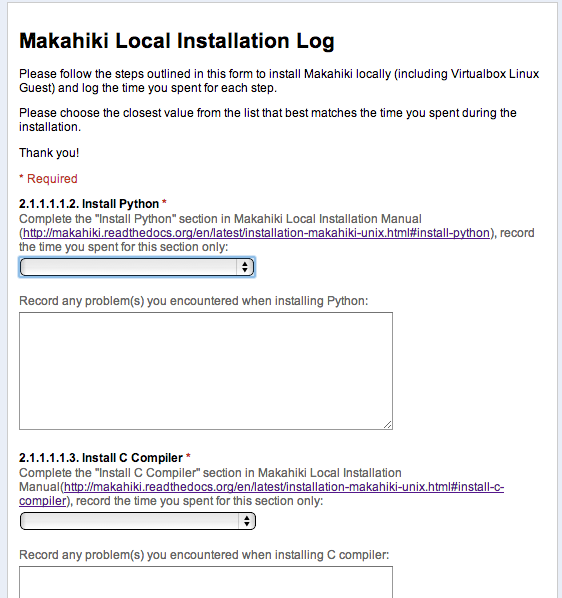
\includegraphics[height=30em,width=30em]{developer-eval-form.png}
   \caption{Makahiki Developer Evaluation Form}
   \label{fig:developer-eval-form}
\end{figure}

I also ask the students to provide feedbacks about their installation experiences in the form of blog post. In the blog post, I ask them to discuss the following topics:
\begin{itemize}
\item What is the most difficult step during installation?
\item What problems did you encounter during the installation?
\item Have you install any database, web server or similar server products prior to this assignment? Are those installations for development or production purpose?
\item If you have experience installing other servers before, How does your prior experience of installing other servers compare to the installation of Makahiki?
\item What could be improved about the Makahiki installation process?
\item Compare your experience of installing Makahiki in Heroku with installing it locally,
\end{itemize}

I will analyze these qualitative data collected from the google form response and the blog post from the students, to gain insights into how easy it is to install Makahiki, and what contributes to the efficiency of the installation.

\subsubsection{Game designer efficiency evaluation}
Another class assignment for students is to design a Kukui Cup like serious game using Makahiki. I designed another google form to ask students to follow the designing steps and record their time and problem encountered during their desiging process. \autoref{app:googleform} has the complete google form for the steps the students need to follow.

I also ask the students to provide feedbacks about their installation experiences in the form of blog post. In the blog post, I ask them to discuss the following topics:
\begin{itemize}
\item What is the most difficult step during Challenge Design?
\item What problems did you encounter while designed the challenge?
\item What problems did you encounter while managing the challenge?
\item What could be improved for the Makahiki Challenge Design process?
\item What could be improved for the Makahiki Challenge Management process?
\end{itemize}

\subsubsection{Developer efficiency evaluation}

The students are tasked with developing an enhancement to the Makahiki instance. This envolves setting up the development environment, following the tutorial to create the "Hello world" widget using Makahiki, and finally, develop the enhancement which extends the functionality of the Makahiki system.

The students are asked to submit their development source code to the public source code repository (Github) and write a blog post to discuss their efforts to complete the development activity.

I will review their source code to compare their code to the reference implementation, analyze the blog post from the students, as well as any email correspondence from students discussing the problem in the development.

\subsubsection{Preliminary Results}

\section{Lucid Design Dashboard evaluation case study}
